\subsection{Checking a card}

The next method we shall model with SDMs is probably the most important: a
user decides to try a card in the memory box and looks at the question on the
card (\texttt{Card.face}), makes a guess and \emph{checks} to see if the guess
was correct by comparing with the answer on the back of the card
(\texttt{Card.back}).  If the guess was correct the card can be \emph{promoted}
by moving it to the \emph{next} partition, if it was wrong the card is
\emph{penalised} by moving it to the \emph{previous} partition.

As you're almost an SDM wizard already, try, using concepts we have
already learnt, to create the control flow for \texttt{Partition::check} as
depicted in Fig.~\ref{fig:sdm_check_start}.

\begin{figure}[htbp]
\begin{center}
  \includegraphics[width=\textwidth]{pics/sdmBilder/check/sdm16RAW.pdf}
  \caption{Activity diagram for \texttt{Partition::check}.}  
  \label{fig:sdm_check_start}
\end{center}
\end{figure}
 
To check if the guess was correct, create an object variable that is bound to
the argument \texttt{card}, representing the card the user has picked from the
memory box.  Remember that this binding is implicitly specified by choosing the
name of the argument as the name of the object variable
(Fig.~\ref{fig:sdm_check_addCard}).

\clearpage

\begin{figure}[htbp]
\begin{center}
  \includegraphics[width=0.85\textwidth]{pics/sdmBilder/check/sdm17RAW}
  \caption{Add the card to be checked.}  
  \label{fig:sdm_check_addCard}
\end{center}
\end{figure}

Now that we have the card to be checked, we need to compare the user's guess to
\note{Attribute Constraint}
the actual answer on the back of the card.  To do this we need to specify an
\emph{Attribute Constraint}.  An attribute constraint is a
non-structural condition that must be satisfied for a story pattern to match,
and can be specified by choosing the \texttt{Attribute Constraint} tab as
depicted in Fig.~\ref{fig:sdm_check_att_constraint}.  In this dialogue, choose
the attribute to be used in formulating the constraint (\texttt{back}) and the
type of \texttt{Expression} used to express the constraint.  As we shall compare
the back of the card with the user's guess, passed in as a parameter, we need a
\texttt{ParameterExpression} to refer to this value.  In the previous section,
we already used parameter expressions to specify the return value in a stop
node.  Now choose the parameter (\texttt{guessed}) and the type of
constraint or \emph{operation} to be executed -- in this case an equality check
(\texttt{==}). Press the button labelled \texttt{Add} and admire your first
attribute constraint (Fig.~\ref{fig:sdm_check_att_constraint})!

\begin{figure}[htbp] 
\begin{center}
  \includegraphics[width=0.7\textwidth]{pics/sdmBilder/check/sdm18RAW}
  \caption{Add an attribute constraint with a parameter expression.}  
  \label{fig:sdm_check_att_constraint}
\end{center}
\end{figure} 

Let's get back to the control flow for a bit.  We need to specify that the card
is to be penalised if the guess was wrong (the story node
\texttt{Check\-If\-Guess\-Is\-Correct} did not match) and to be promoted if it
was correct (a match could be found, i.e., all constraints/conditions both
\note{Edge Guards}
structural and non-structural could be fulfilled).  Such an if/else construct is
specified in SDMs via \emph{Edge Guards}.  To add a guard to the edge leading
from \texttt{Check\-If\-Guess\-Is\-Correct} to \texttt{penalize\-Card}, double
\note{Guard Type}
click the edge and choose the \emph{Guard Type} in the dialogue
(Fig.~\ref{fig:sdm_check_guard}).  Choose \texttt{Failure}, repeat the process
for the edge leading to \texttt{promoteCard} and choose \texttt{Success}.

\begin{figure}[!htbp]
\begin{center}
  \includegraphics[width=0.6\textwidth]{pics/sdmBilder/check/sdm19}
  \caption{Add a transition with a guard.}  
  \label{fig:sdm_check_guard}
\end{center}
\end{figure}

\clearpage 

The next feature of our tool we shall learn is a means of coping with large
patterns.  It might be nice to visualise \emph{small} story patterns directly in
their story nodes, but for large patterns or complex surrounding control flow,
such diagrams would get very cumbersome and unwieldy pretty quickly.  This is
indeed a popular argument against visual languages and it might already have
crossed your mind (``this is cute, but it'll \emph{never} scale!'').  With the
right tools and concepts however, even huge diagrams can be mastered.  We
\note{Extracting Patterns}
support \emph{extracting} story patterns to their own extra diagrams and
recommend this for most cases (unless the pattern is really concise and
only contains about 2-3 object variables).  

\begin{figure}[htbp]
\begin{center}
  \includegraphics[width=0.7\textwidth]{pics/sdmBilder/check/sdm21}
  \caption{Extract a story pattern for more space and a better overview.}  
  \label{fig:sdm_check_extract_storypattern}
\end{center}
\end{figure}

To extract an empty or already
partially modelled story pattern, just double-click the corresponding story node
(\texttt{promoteCard}) and choose \texttt{Extract Story Pattern}
(Fig.~\ref{fig:sdm_check_extract_storypattern}). Note the new diagram that is
immediately opened and created in the project browser
(Fig.~\ref{fig:sdm_check_bound_card}).
\clearpage

\begin{figure}[htbp]
\begin{center}
  \includegraphics[width=0.8\textwidth]{pics/sdmBilder/check/sdm22RAW}
  \caption{Add an object variable per drag and drop.}  
  \label{fig:sdm_check_bound_card}
\end{center}
\end{figure}

Yet another EA gesture is good old \emph{Drag and Drop} from the project
\note{Drag \& Drop}
browser\footnote{Remember the other two gestures we have learnt:  Quick Link
and Quick Create.}, which we use as an alternative to the SDM toolbox.  
To create an object variable, simply drag and drop the class
\texttt{Card} from the project browser and into the extracted story
pattern diagram (Fig.~\ref{fig:sdm_check_bound_card}).  A dialogue should pop-up
asking if you want to (1) create a simple link (referring to \texttt{Card} as a
class) or (2) create an Object (as an instance of \texttt{Card}), or (3), if you
want to create a subclass.  In our case we want to create an object(variable) 
and so (2) is nearest in meaning.  As this \texttt{Paste Element} dialogue is a
bit annoying, EA  allows you to choose a default for \emph{all} drag and drop
gestures.  Go ahead and check \texttt{All Drag and Drop} so that option (2) is
used next time as the default.  Furthermore, you should also check 
\texttt{Only show this dialog when Ctrl+Mouse drag is used}, so that the 
default is used \emph{without} popping up this dialogue for confirmation. Don't worry,
if you ever need options (1) and (3), for example when metamodelling, you  just
need to hold \texttt{Ctrl} when dragging to invoke the dialogue and change  the
settings to suit the current modelling activity. 

The main advantage of drag and drop is that the \texttt{Object Variable
Pro\-per\-ties} dialogue that now pops-up should have the type of the object
variable pre-configured. Choosing the type in the project browser and dragging it in
is for most people a more natural gesture than choosing the type from a long
drop-down menu and can really be a great time saver for large
metamodels\footnote{Drag and drop is also possible in embedded story patterns
(still visualised in their story nodes).  You must ensure however, that the
object variable is \emph{completely} contained inside the story node and does
not stick out over any edge}. 

Let's move on with the current pattern. Remember that we want to promote the
card.  As a first step drag and drop two further object variables for
\texttt{this} (the current partition) and the next partition according to
(Fig.~\ref{fig:sdm_check_complete_sp}).  An important point to note here is
that \texttt{this} and \texttt{card} are visually differentiated from
\texttt{nextPartition} by their bold border lines. This is how we differentiate
\emph{bound} \note{Bound vs. Unbound} variables (\texttt{this, card}) from
\emph{unbound} or \emph{free} variables like \texttt{nextPartition}.  We already know that matches for bound variables are completely determined by the current
context (argument of the method, current ``this" object).  Matches for unbound
variables on the other hand, have to be determined by the pattern matcher.  Such
matches are ``found'' by navigating and searching in the current model for
possible matches that satisfy all specified constraints (e.g. type of the
variable, links connecting it to other variables and attribute constraints). 

\begin{figure}[htbp]
\begin{center}
  \includegraphics[width=0.7\textwidth]{pics/sdmBilder/check/sdm25.pdf}
  \caption{All object variables for story pattern \texttt{promoteCard}.}  
  \label{fig:sdm_check_complete_sp}
\end{center}
\end{figure} 

In our case, the next partition has to be determined, by navigating from
\texttt{this} via the \texttt{next} link in the metamodel.  Make sure the bound
checkbox for \texttt{nextPartition} is left empty and quick link from
\texttt{this} to \texttt{nextPartition}, or vice-versa, to create a
\texttt{next} link variable as indicated in
Fig.~\ref{fig:sdm_check_link_variable}. 

\begin{figure}[htbp]
\begin{center}
  \includegraphics[width=0.6\textwidth]{pics/sdmBilder/check/sdm26}
  \caption{Create a link variable.}  
  \label{fig:sdm_check_link_variable}
\end{center}
\end{figure}

If you've done everything right, your story pattern should now closely resemble
Fig.~\ref{fig:sdm_check_complete_activity_node}.  Take a step back and reflect
on what the pattern expresses.

\clearpage

\begin{figure}[htbp] 
\begin{center}
  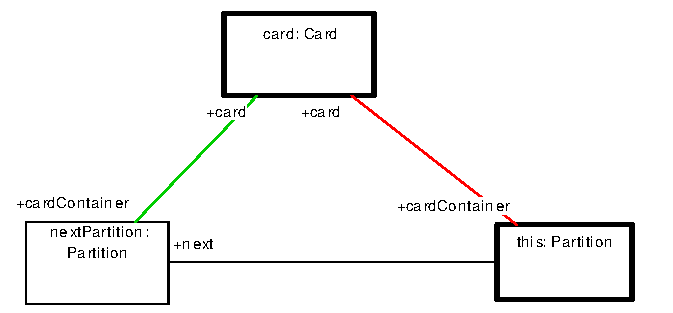
\includegraphics[width=0.6\textwidth]{pics/sdmBilder/check/sdm30}
  \caption{Complete story pattern for activity node \texttt{promoteCard}.}  
  \label{fig:sdm_check_complete_activity_node}
\end{center}
\end{figure}

Now repeat the process for the story node \texttt{penalizeCard}: extract the
story pattern, and create all variables as depicted in
Fig.~\ref{fig:sdm_check_complete_penalize}.  This pattern is quite similar to
\texttt{promoteCard} but moves the card from \texttt{this} to \texttt{previous}
instead of \texttt{next}.  Just like before, \texttt{previousPartition} is
unbound and must be determined by navigating from \texttt{this} along the link
\texttt{previous}.

\begin{figure}[htbp]
\begin{center}
  \includegraphics[width=0.6\textwidth]{pics/sdmBilder/check/sdm38}
  \caption{Story pattern for activity node \texttt{penalizeCard}.}  
  \label{fig:sdm_check_complete_penalize}
\end{center}
\end{figure}

To complete our SDM, we need to signalise, as a return value, if the guess was
correct or not (and consequently if the card was promoted or penalised).  To do
\note{Literal Expression}
this, double-click the stop node after \texttt{promoteCard} and choose
\texttt{LiteralExpression} as the type of expression
(Fig.~\ref{fig:sdm_check_literal_exp}).  

\begin{figure}[htbp]
\begin{center}
  \includegraphics[width=0.6\textwidth]{pics/sdmBilder/check/sdm39}
  \caption{Add a return value with a literal expression.}  
  \label{fig:sdm_check_literal_exp}
\end{center}
\end{figure}

\emph{Literal expressions} can be used
to specify arbitrary text.  This should actually be used only for
\emph{literals} like 42, ``foo'' or \texttt{true} but can of course be (mis)used
for formulating any (Java) expression that will simply be transferred
``literally'' into the  generated code. This is obviously sort of
dirty\footnote{It defeats, for example, any attempt to guarantee type safety.} 
and should be avoided if possible.
  
\begin{figure}[htbp]
\begin{center}
  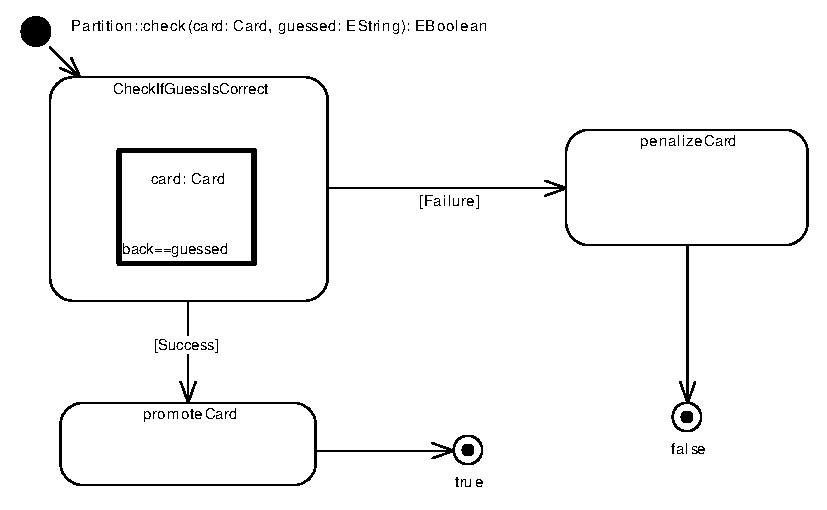
\includegraphics[width=0.7\textwidth]{pics/sdmBilder/check/sdm40}
  \caption{Complete SDM for \texttt{Partition::check}.}  
  \label{fig:sdm_check_finish}
\end{center}
\end{figure}

\clearpage

Type in \texttt{true} as the value of the expression
(Fig.~\ref{fig:sdm_check_literal_exp}) and complete the SDM by returning
\texttt{false} after penalising a card.  Please ensure that your SDM (the
control flow) closely resembles Fig.~\ref{fig:sdm_check_finish}.  As always,
export the project, generate code and inspect the implementation for
\texttt{check}.  We strongly recommend that you even write a simple JUnit test
(take a look at our simple test case in Sec.~\ref{sec:junit} for inspiration)
to take your brand new SDM for a test-spin.
